%----------------------------------------------------------------------------------------
%	PACKAGES AND OTHER DOCUMENT CONFIGURATIONS
%----------------------------------------------------------------------------------------

\documentclass[11pt, notitlepage]{article} % Default font size and suppress title page

\usepackage[utf8]{inputenc} % Required for inputting international characters
\usepackage[T1]{fontenc} % Output font encoding for international characters
% A note on fonts: As of 2019, NIH allows Arial, Georgia, Helvetica, and Palatino Linotype. Georgia and Arial are commercial fonts so you will need to use XeLaTeX and have them installed on your machine to use them. Palatino & Helvetica are available as free LaTeX packages so select the one you want and comment out the other.
\usepackage{palatino} % Palatino font
\linespread{1.05} % A little extra line spread is better for the Palatino font
%\usepackage{helvet} % Helvetica font
\renewcommand*\familydefault{\sfdefault} % Use the sans serif version of the font

\usepackage{amsfonts, amsmath, amsthm, amssymb} % For math fonts, symbols and environments
\usepackage{graphicx} % Required for including images
\usepackage{booktabs} % Nice rules in tables
\usepackage{wrapfig} % Required for text to wrap around figures and tables
\usepackage[labelfont=bf]{caption} % Make figure numbering in captions bold
\usepackage[top=0.5in,bottom=0.5in,left=0.5in,right=0.5in]{geometry} % Page margins
\pagestyle{empty} % Suppress headers and footers

\hyphenation{ionto-pho-re-tic iso-tro-pic fortran} % Specifies custom hyphenation points for words or words that shouldn't be hyphenated at all

%----------------------------------------------------------------------------------------

\begin{document}

%----------------------------------------------------------------------------------------
%	GENERAL INFORMATION
%----------------------------------------------------------------------------------------

\begin{center}
{\Large \textbf{Project Description:}}\\  
\vspace{.5cm}
{\LARGE\textbf{Project Name}} 
\\[.75cm] 
submitted by\\
{Yernur Baibolatov\\
Universit\"at Potsdam\\
Institut f\"ur Physik und Astronomie}
\end{center}
%\\[.75cm] 
\noindent\textbf{Specific academic field (specialization)}: Planetology?
\\[.75cm] 
\textbf{Supervisor and first expert reviewer for recommendation letters}: Prof. Dr. Frank Spahn
\\[.75cm] 
\textbf{Further expert reviewers (name, academic field; these do not have to be identical with the second reviewer of the PhD thesis)}: ???
\\[.75cm] 
\textbf{Working environment}: Please  briefly  explain  how you  are  integrated  in  colloquia, a  working  group,   a  research  training group etc.  Please indicate if you are an individual doctoral student.

\section*{Abstract}
Clear  and  comprehensible  presentation  of  the  project,  short  characterization  of  your  project’s  objectives (not longer than 15 lines)


%----------------------------------------------------------------------------------------
%	Summary of the research topic
%----------------------------------------------------------------------------------------

\newpage

\section*{A. Summary of the research topic}

The model we consider is a granular gas with polydisperse size-distribution 
of constituents in a sheared environment. In our further discussion, we will be
using the term \emph{granular temperature} or simply \emph{temperature}, 
referring to the mean kinetic energy of constituents, and not molecular heat energy.

Unlike molecular gases, a granular gas is always subject to dissipation of inner 
energy or temperature decay over time \cite{Haff1983,Brilliantov2004}. Even more interesting phenomena can be
observed when granular gas consists of species with different masses. In this case, 
due to non-equal partitioning of energy, each species attain unique granular 
temperatures \cite{Garzo2007c,Osinsky2020}. 
The time evolution of these temperatures is in the next form:
\begin{equation}
	\frac{dT_i}{dt} \propto H_i -A_iT_i+\sum_{k}B_{ik}(T_i-T_k)\;,
\end{equation}
where $T_i$ and $T_k$ are granular temperatures, $A_i>0$ is the parameter describing 
dissipation due to collisions, which depends on size distribution function, collision 
frequency and restitution. The parameter $B_{ik}=B_{ki}>0$ describes the inter-species 
heat flow. This is the main reason why species tend to have different temperatures. 
$H_i$ is a certain external heating function. If one introduces an external energy pump 
into the system, the temperatures of species don't reach zero, but attain certain 
stationary and still unique values, balancing the outer heating \cite{Bodrova2014}. 

One caveat of these heating models is that they are all artificial. Our goal 
is to investigate the model with a more realistic heating term, the gravitational 
shear heating in planetary disks. This heating is in the next form:
\begin{equation}
	H_i \propto \nu_i\Omega^2\;,
\end{equation}
where $\Omega$ is the mean orbital frequency around the considered location of the system,
and $\nu_i$ is the shear viscosity term. In the case of planetary rings, the viscosity
term is split into \emph{local} and \emph{non-local} parts $\nu=\nu_l+\nu_{nl}$ \cite{Seiss2011,Spahn2006,Stewart1984}.
However, these terms are given only for the mono-disperse case. In the case of a gas 
with different species, we need to know the viscosity terms for each species. 
This is the first goal of our project, to obtain the kinetic transport coefficients
for each species from the microscopic level of description. 
By this we mean kinetic description of the system, given a velocity distribution 
function $f$, its time evolution obeys:
\begin{equation}
	\frac{\partial f_i}{\partial t}+\vec{v}\cdot\frac{\partial f_i}{\partial\vec{r}}-
	-\frac{1}{m_i}\frac{\partial U}{\partial\vec{r}}\frac{\partial f_i}{\partial\vec{v}}=
	\sum_k\eta_kI(f_i,f_k)\;,
\end{equation}
where $I(f_i, f_k)$ is the collision integral and $\eta$ is the size distribution 
function.

In order to test the theoretical results, we have developed a molecular dynamics (MD) 
code, simulating granular particles of different sizes in a Hill's box. 
\emph{Here some $\ln T$ over $\ln t$ simulation results graph Fig.~\ref{fig2}}
\begin{figure}[h] % Figure at bottom of the page ([b] argument, could be "t" for top or "h" for here)
	\centering
	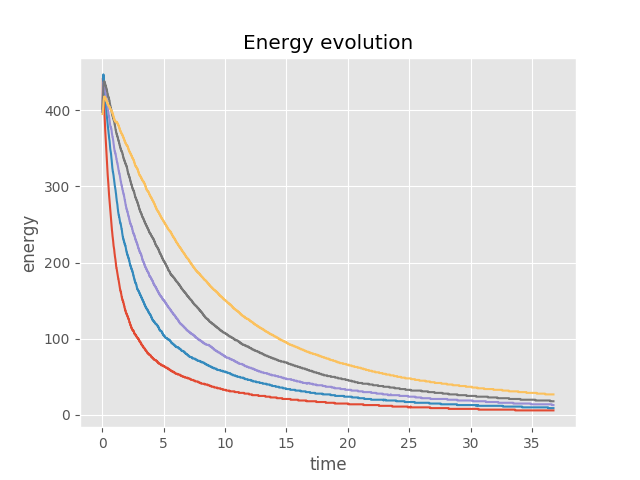
\includegraphics[scale = .80]{Figures/energy_evo.png}
	\caption{\footnotesize This is only an example plot. Should be replaced by my new simulation results}
	\label{fig2}
\end{figure}

Next, we would like to address the reasons for size distribution in Saturn's rings. 
From experimental evidence, we that the size distribution obeys a power
law with a cut-off at the end [size-distribution tail original works]. There are several attempts
to model this phenomenon \cite{Brilliantov2013,Spahn2011}. All of them assume a certain interplay between
two driving processes, aggregation or coagulation process when particles merge, producing 
larger particles, and fragmentation process, when particles
fracture after collision producing smaller constituents. A natural step for us would be 
to analyze the kinetic equations describing the behavior of the system with inclusion 
of aggregation and fragmentation processes.

Such an interplay and balance of three different processes, one being separation of 
temperatures of species, second being the gravitational heating and third 
being the recombination of particles which lead to dynamical change of size distribution,
is already quite interesting. Hence, an external influence, such as periodic 
driving force acting upon the system should lead to various fascinating phenomena.
In planetary systems, such periodic driving forces are resonances with the moons of the 
planet.

%----------------------------------------------------------------------------------------
%	Table of contents and outline of the thesis with an overview of accomplished (sub-) chapter
%----------------------------------------------------------------------------------------

\newpage
\section*{B.Table of contents and outline of the thesis with an overview of accomplished (sub-) chapter}
Please submit your table of contents /outline of your thesis. Please characterize the (sub-)chapter that have already been accomplished. The probability of concluding the project during the funding period  must  be  illustrated.  The awarding committee reserves the right to obtain the stated (sub-) chapter in printed form.

%----------------------------------------------------------------------------------------
%	Working program and intended completion date
%----------------------------------------------------------------------------------------

\newpage
\section*{C. Working program and intended completion date}
\begin{itemize}
    \item Working-Program, time schedule (max. 4 pages)Detailed information about your planned approach, especially a thorough explanation of the meth-odology, that you will apply in the completion phase of your  PhD. A time schedule (e. g. in graphic or  tabular  form)  for  the  period  of  funding  should  clearly  demonstrate  the  steps  in  your  research  project that are planned, have already started or are completed. If your PhD includes experiments, please indicate the experiments that have already been conducted and that will still be conducted. The  quality  of  the  research  approach  and  the  characterization  of  the  accomplished  and  planned  steps are of utmost importance.
    \item Please specify your intended completion date.
\end{itemize}
%----------------------------------------------------------------------------------------
%	Literature
%----------------------------------------------------------------------------------------

\newpage
\section*{D. Literature}

\newpage

\bibliography{project} % Use the NIHGrant.bib file for the reference list, replace with your own
\bibliographystyle{nihunsrt} % Use the custom nihunsrt bibliography style included with the template

%----------------------------------------------------------------------------------------

\end{document}